\documentclass{beamer}
\usepackage[francais]{babel}
\usepackage[T1]{fontenc}
\usepackage[utf8]{inputenc}  
\usepackage{verbatim} 
\usepackage{indentfirst}          %pour \verbatiminput{fich}
\usetheme{JuanLesPins}    % titre en haut
%\useoutertheme{default}       
\setlength{\parindent}{0.5cm}

\graphicspath{{Figures/}}
\setbeamertemplate{caption}[numbered] % pour numéroter tables et figures !
%si \verb   : \begin{frame}[fragile]
%si verbatim  : \begin{frame}[containsverbatim]


\title{Robotique, état de l'art}
\author{Jérémy SIMIONE, Thomas BESSON , Leif HENRIKSEN}
\institute{Université de Montpellier}
\date{2019}

\begin{document}
% Premier transparent de titre
\begin{frame}
  \titlepage
\end{frame}

\begin{frame}
  \frametitle{Sommaire}
  {\small \tableofcontents}
\end{frame}

\section{Definitions, Intérêts, Historique et Composition d'un Robot}
\subsection{Definitions}

\begin{frame}
  \frametitle{Definitions}
  
\begin{block}{Robot}
Appareil automatique capable de manipuler des objets ou d'exécuter des opérations selon un programme fixe, modifiable ou adaptable.
\end{block}

\begin{block}{Robotique}
Science et technique de la robotisation, de la conception et de la construction des robots.
\end{block}

\begin{block}{Bot}
 Programme informatique automatisant des tâches répétitives, ou mimant le comportement d’un être humain.
\end{block}
\end{frame}




\subsection{Origine du mot}
\begin{frame}
  \frametitle{Origine du mot Robot}
	\begin{itemize}
		\item Il fut initialement utilisé par l’écrivain tchécoslovaque Karel Čapek dans sa pièce de théâtre R. U. R. 		(Rossum's Universal Robots) en 1920. Cette pièce fut jouée pour la première fois en 1921. Bien que Karel Čapek soit souvent considéré comme l’inventeur du mot, il a lui-même désigné son frère Josef, peintre et écrivain, comme étant l’inventeur réel du mot.
	
		\item  Les « robots » de Karel Čapek étaient des humains organiques artificiels.
	\end{itemize}
\end{frame}

\subsection{Intérêts de la robotique}
\begin{frame}
  \frametitle{L'idee de la Robotique}
  
  \begin{block}{Aristote, La Politique, livre 1, chapitre 4}
  <<En effet, si chaque outil pouvait, lorsqu’on le lui commanderait, ou même en pressentant d’avance l’ordre, exécuter, la tâche qui lui est propre, comme faisaient, dit-on, les statues de Dédale, ou comme les trépieds de Vulcain, qui d’eux-mêmes entraient, comme dit le poète, dans le conseil des dieux : si donc la navette… pouvait ainsi ; d’elle-même tisser la toile, ou l’archet frapper les cordes de la cithare, alors ni les  architectes n’auraient besoin de manœuvre, ni les maîtres n’auraient besoin d’esclaves ...>> 
  \end{block}

\end{frame}

\subsection{Historique}


\begin{frame}
  \frametitle{Automates}
  
  \begin{block}{Automate}
 Un automate est un dispositif reproduisant en autonomie une séquence d'actions prédéterminées sans l'intervention humaine, le système fait toujours la même chose.
\end{block}

\begin{block}{Automate vs Robot}
  Le automate obéit à un programme strictement préétabli, que ce soit de manière mécanique ou électrique, alors que le robot dispose de capteurs et d'appareillages électroniques, de sorte que ses actions découlent de ses contacts avec son environnement, ce qui - à la différence de l'automate - le rend autonome, "intelligent".
\end{block}

\end{frame}

\begin{frame}
  \frametitle{Exemple d'Automate}
  \begin{figure}[!h]
  \centering
  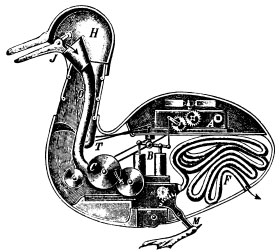
\includegraphics[width=6cm]{Duck_of_Vaucanson.jpg}
  \caption{Le Canard digérateur par Jacques de Vaucanson en 1738}
  \end{figure}
\end{frame}

\begin{frame}
  \frametitle{20 siecle}
  \begin{figure}[!h]
  \centering
  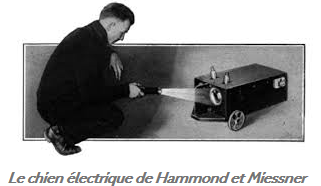
\includegraphics[width=6cm]{chien-electrique-hammond-miessner.png}
  \caption{Le chien électrique, John Hammond et Benjamin Miessner, 1915}
  \end{figure}
\end{frame}

\begin{frame}
  \frametitle{20 siecle}
  \begin{figure}[!h]
  \centering
  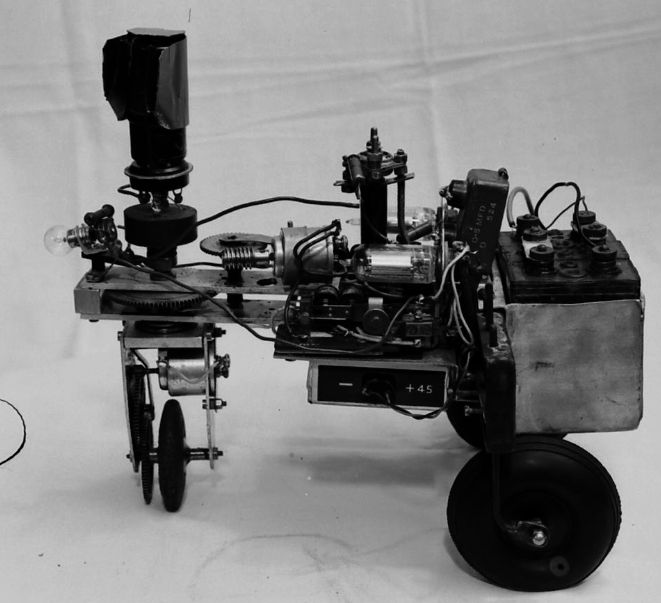
\includegraphics[width=6cm]{ELSIE-Time-Life1950.jpg}
  \caption{Les tortues cybernétiques de William Grey Walter, 1950}
  \end{figure}
\end{frame}

\begin{frame}
  \frametitle{Premier Robot Industriel}
  \begin{figure}[!h]
  \centering
  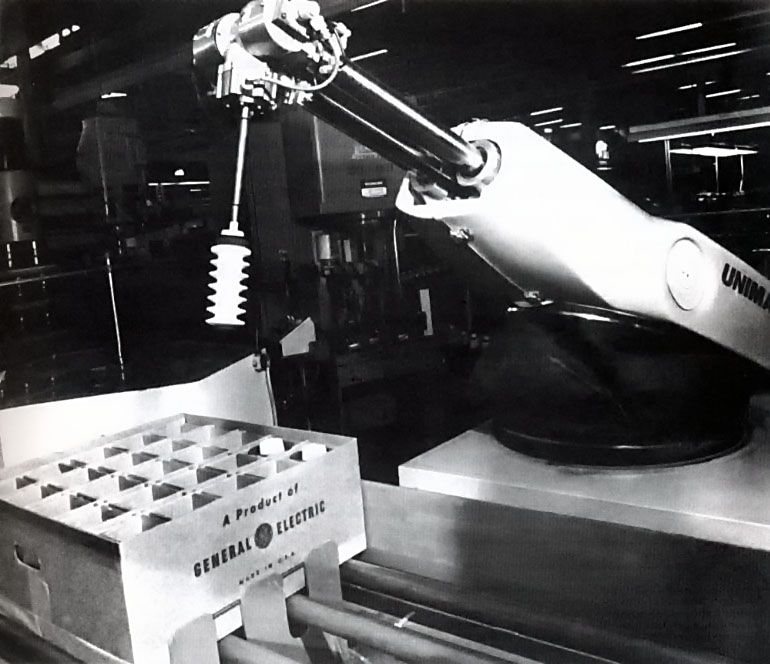
\includegraphics[width=6cm]{1961.jpg}
  \caption{Le Unimate, 1961}
  \end{figure}
\end{frame}
  
\begin{frame}
 \frametitle{Premier Robot Industriel}
  \begin{figure}[!h]
  \centering
  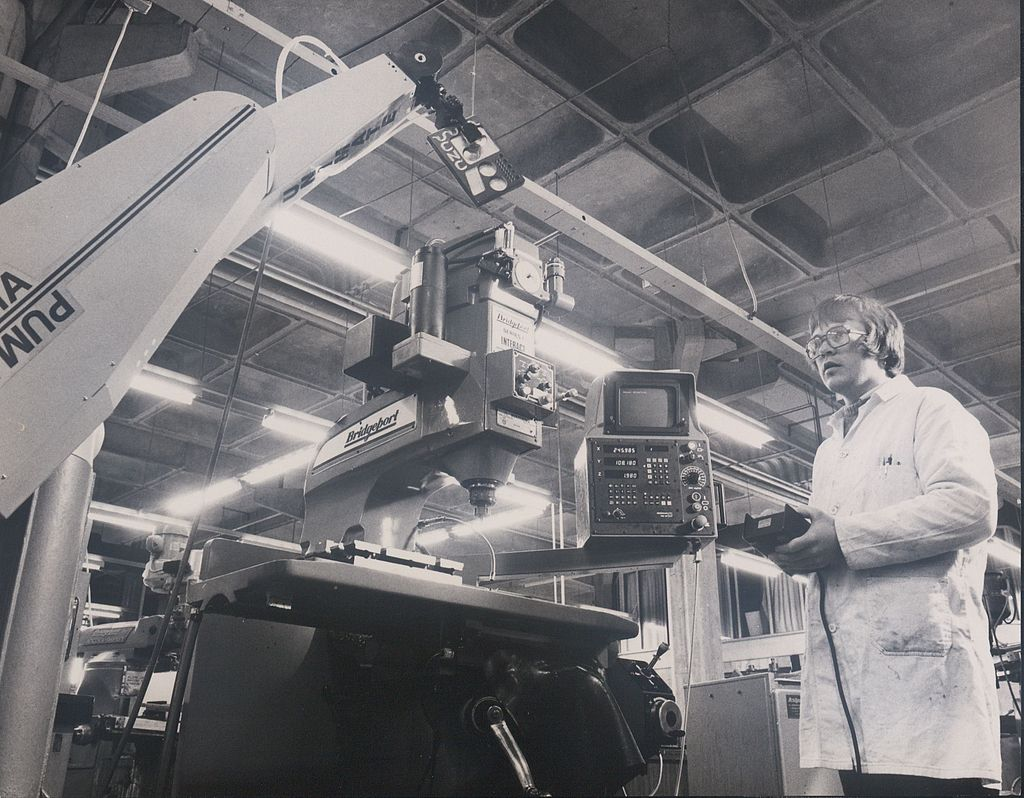
\includegraphics[width=6cm]{pumo2.jpg}
  \caption{Le Unimate 25 ans apres}
  \end{figure}
\end{frame}

\begin{frame}
  \frametitle{Premiers Robots Militaires}
  
  \begin{figure}[!h]
  \centering
  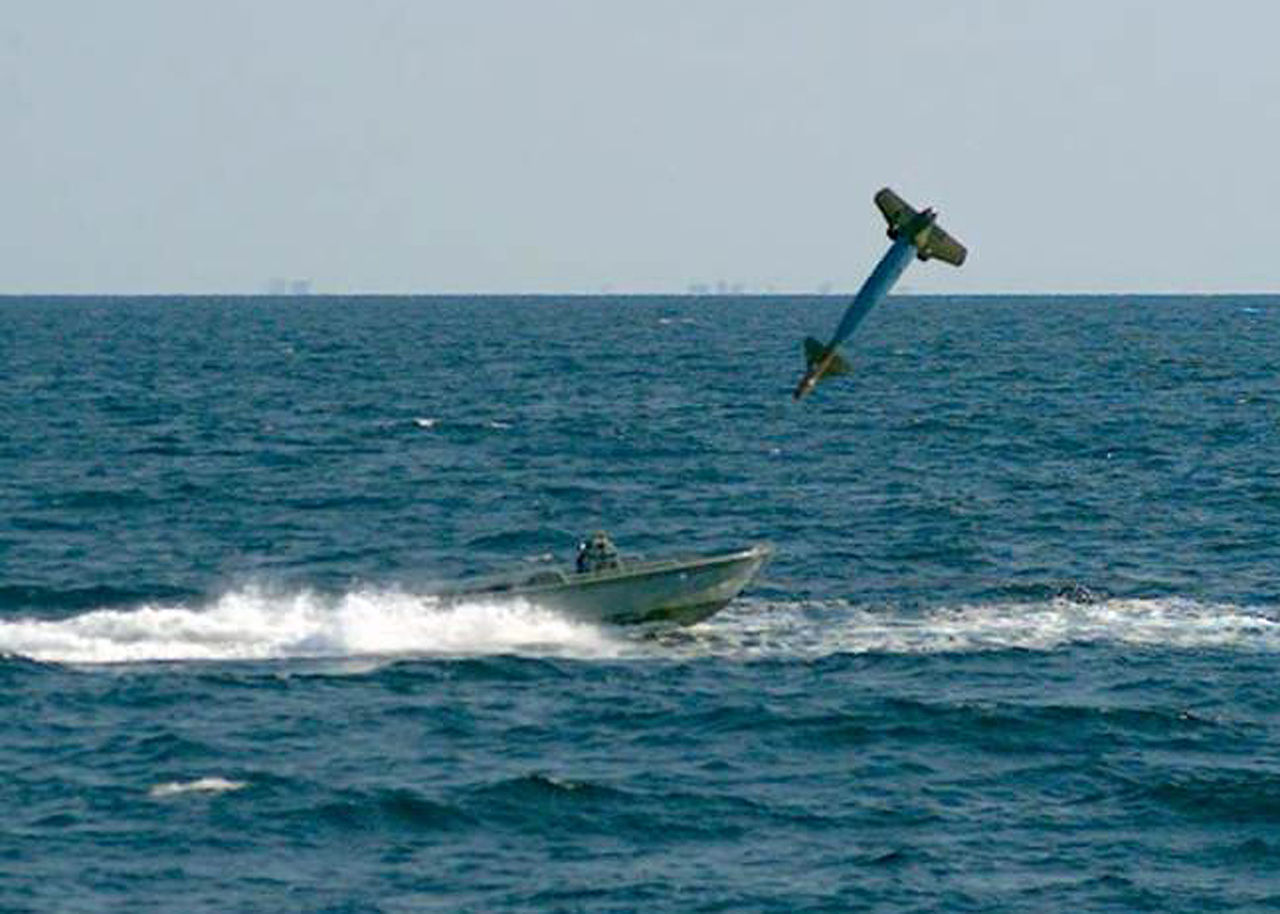
\includegraphics[width=6cm]{1280px-GBU-10_shortly_before_it_impacts_a_small_boat_during_a_training_exercise.jpg}
  \caption{GBU-10 Paveway II, bombe americaine guide par laser}
  \end{figure}
  
\end{frame}

\begin{frame}
  \frametitle{21 siecle}
  \begin{figure}[!h]
  \centering
  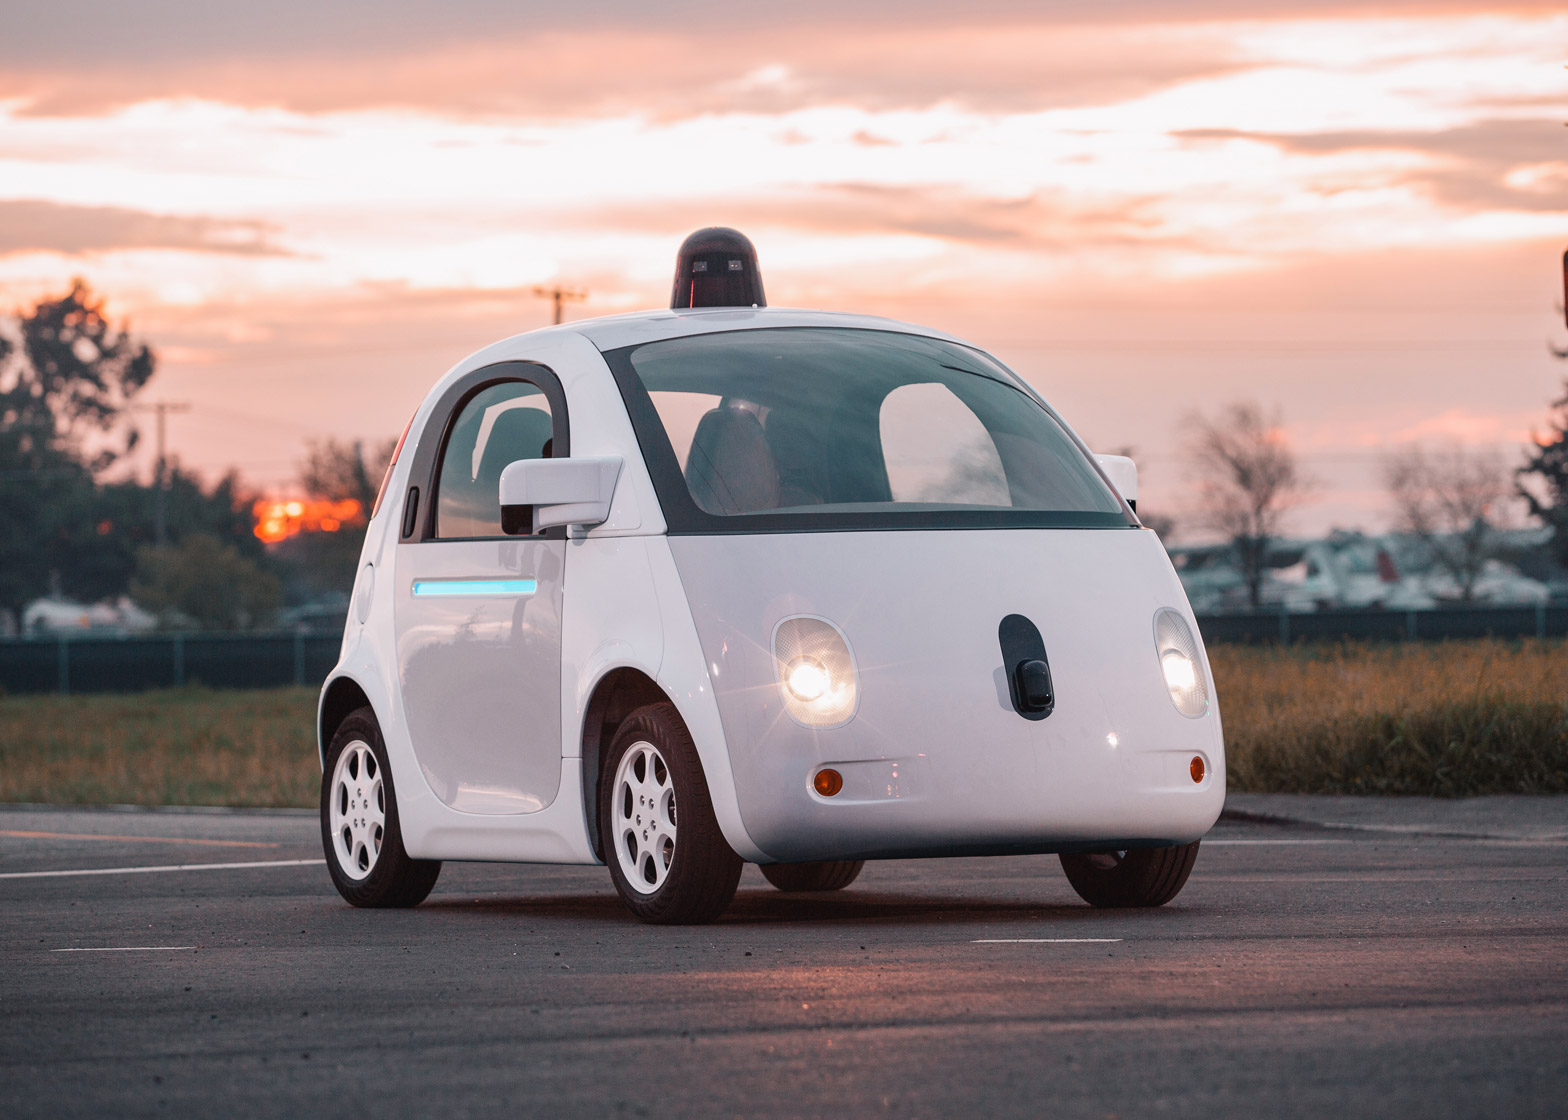
\includegraphics[width=6cm]{google-artificial-intelligence-first-non-human-driver_dezeen_1568_1.jpg}
  
  \end{figure}
\end{frame}

\begin{frame}
\frametitle{DARPA Grand Challenge}
\begin{itemize}
      \item Prix 1.000.000 \$
      \item Premier challenge en 2004, distance maximale parcouru 11.78km 
      \item Deuxieme challenge en 2005, gagnant Stanford avec 212km en 6h54m 
      \item Challenge Urbain en 2007, gagnant Carnegie Mellon University
  \end{itemize}
\end{frame}

\begin{frame}
  \frametitle{DARPA Grand Challenge}
  \begin{figure}[!h]
  \centering
  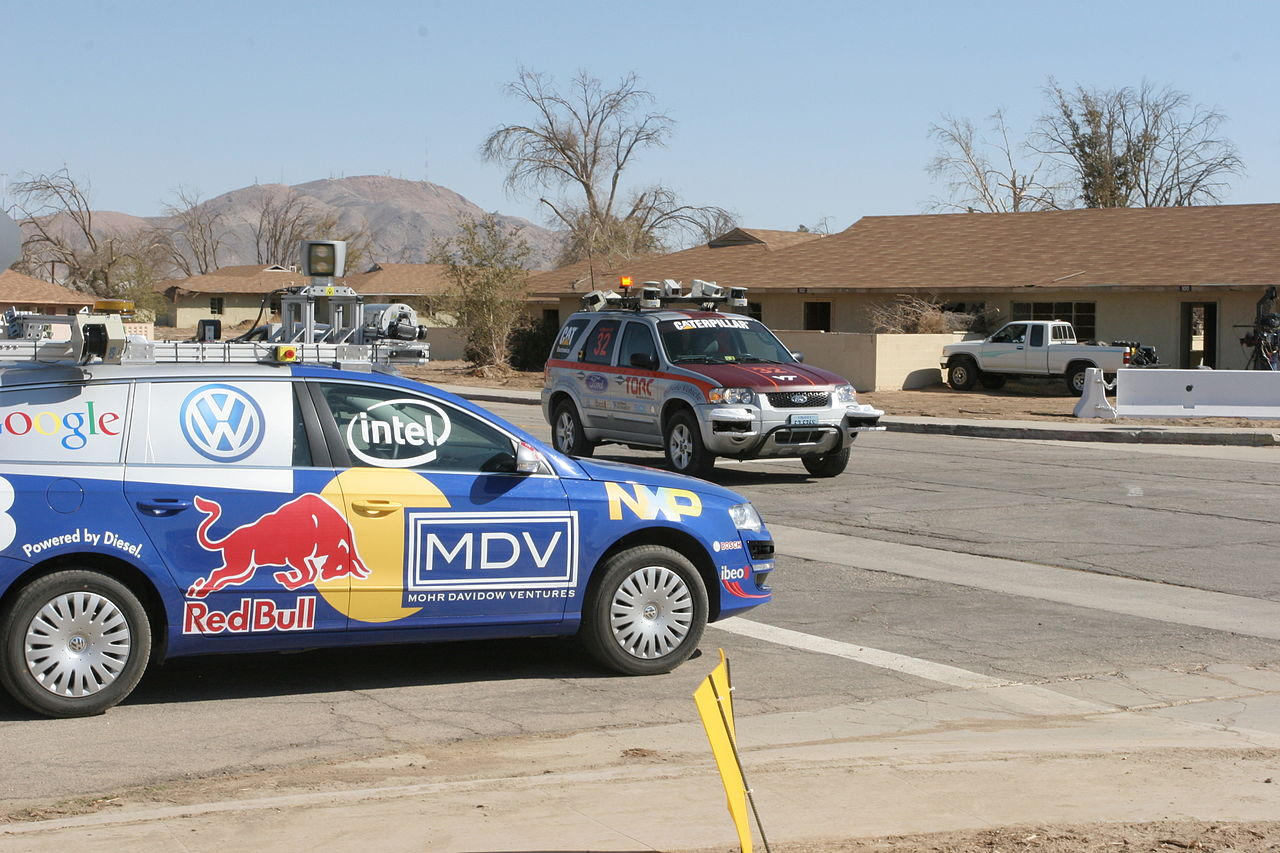
\includegraphics[width=6cm]{1280px-UrbanChallenge_StandfordRacingandVictorTango.jpg}
  \caption{Urban Challenge 2007}
  \end{figure}
\end{frame}

\begin{frame}
\frametitle{Robots pour les particuliers}
\begin{itemize}
      \item Baise des prix
      \item Robots tres faciles a utiliser 
  \end{itemize}
\end{frame}

\begin{frame}
  \frametitle{Robots pour les particuliers}
  \begin{figure}[!h]
  \centering
  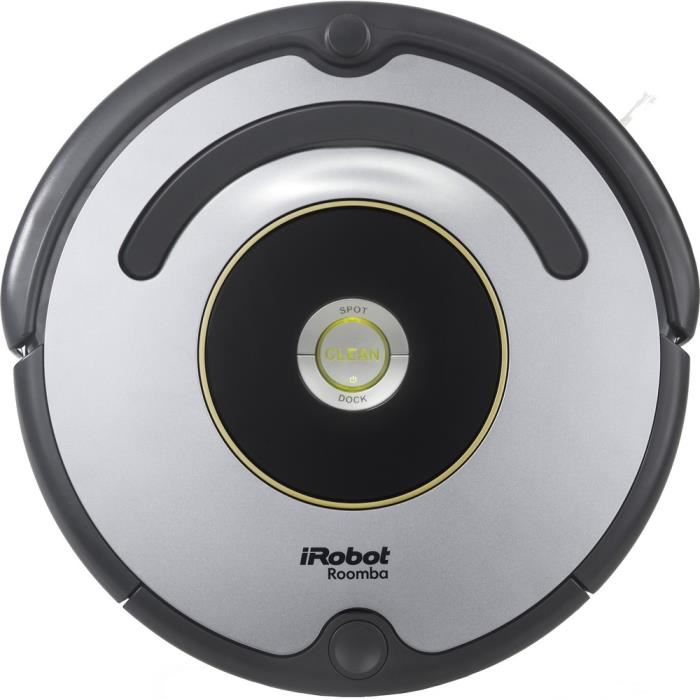
\includegraphics[width=6cm]{irobot-roomba-615-aspirateur-robot-33w-61-db.jpg}
  \caption{Robot Aspirateur}
  \end{figure}
\end{frame}

\begin{frame}
  \frametitle{Robots pour les particuliers}
  \begin{figure}[!h]
  \centering
  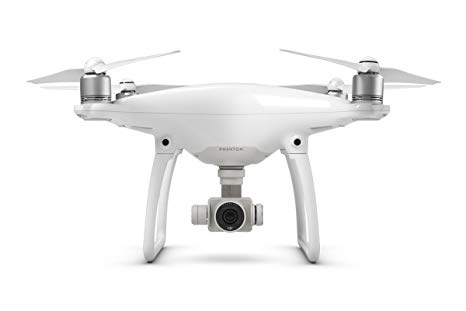
\includegraphics[width=6cm]{drone.jpg}
  \caption{Drone}
  \end{figure}
\end{frame}

\begin{frame}
  \frametitle{Aujourd'hui}
  \begin{figure}[!h]
  \centering
  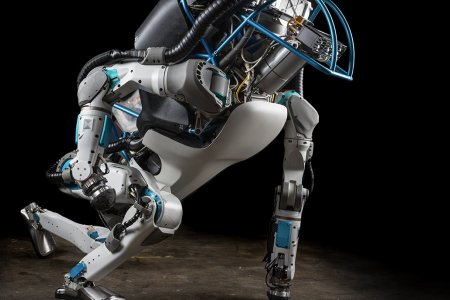
\includegraphics[width=6cm]{header-bkg-atlas_0.jpg}
  \caption{Atlas}
  \end{figure}
\end{frame}



\subsection{Composition D'un Robot}
\begin{frame}
  \frametitle{Structure Mecanique}
  \begin{block}{ }
  La structure mechanique d'un robot est determine par son objective.
  \end{block}
  \begin{block}{Description Technique d'un Robot Industriel}
  \begin{itemize}
      \item Degrees de Liberte
      \item Capacite de transport
      \item Accélération 
      \item Précision
      \item Répétabilité
  \end{itemize}
  \end{block}
\end{frame}

\begin{frame}
  \frametitle{Servos}
  \begin{block}{Définition Servomoteur}
  Un servomoteur est un système motorisé capable d'atteindre des positions prédéterminées, puis de les maintenir. La position est : dans le cas d’un moteur rotatif, une valeur d'angle et, dans le cas d’un moteur linéaire une distance. 
  \end{block}
\end{frame}

\begin{frame}
  \frametitle{Capteurs}
  \begin{block}{Definition}
  Dispositif permettant de capter un phénomène physique et de le restituer sous forme de signal.
\end{block}
\begin{block}{Types de Capteurs}
  \begin{itemize}
      \item Lumiere
      \item Position
      \item Presion
      \item Vitesse
      \item ...
  \end{itemize}
\end{block}
\end{frame}

\begin{frame}
  \frametitle{Gyroscope}
  \begin{figure}[!h]
  \centering
  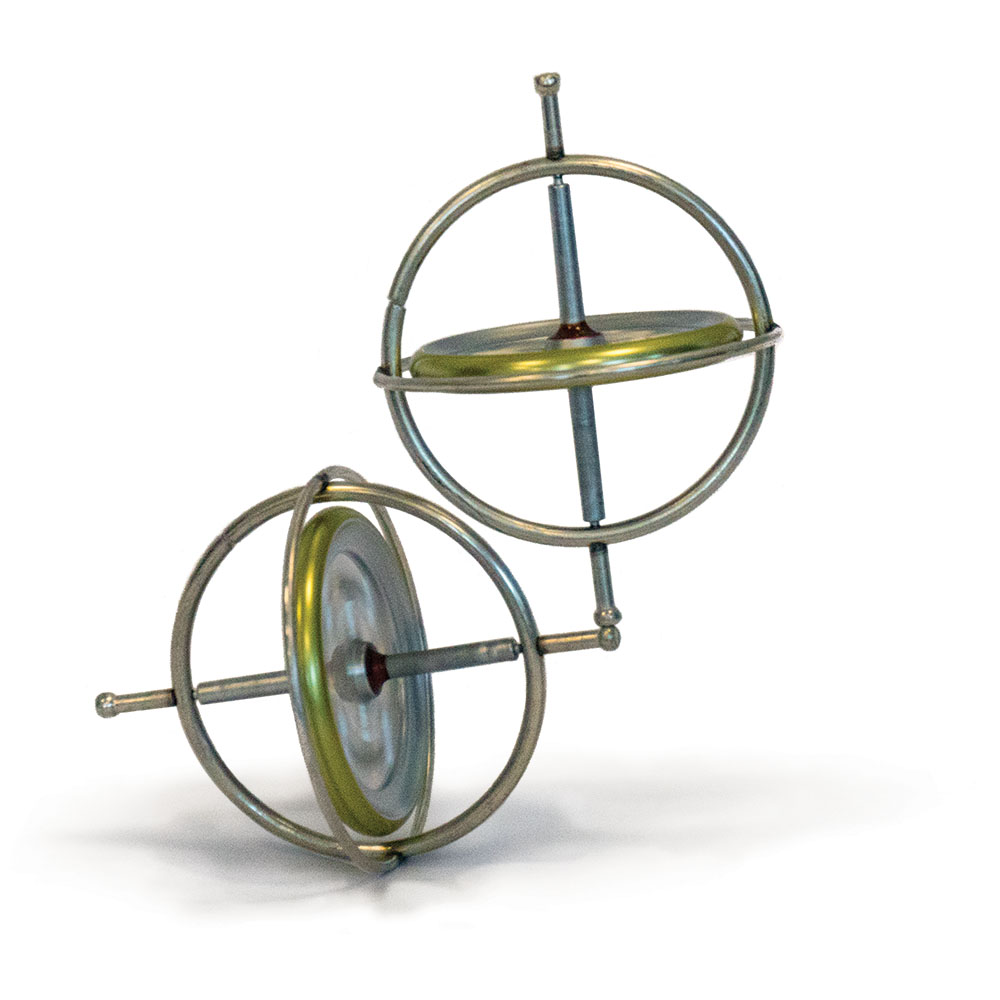
\includegraphics[width=6cm]{000066-twin-gyroscope-gallery-11.jpg}
  \caption{Gyroscope}
  \end{figure}
\end{frame}

\begin{frame}
  \frametitle{Capteur LIDAR}
  \begin{block}{LIDAR}
  \begin{itemize}
  \item La télédétection par laser ou lidar, acronyme de l'expression en langue anglaise « light detection and ranging » ou « laser detection and ranging », est une technique de mesure à distance fondée sur l'analyse des propriétés d'un faisceau de lumière renvoyé vers son émetteur.
  \item À la différence du radar qui emploie des ondes radio ou du sonar qui utilise des ondes acoustiques, le lidar utilise de la lumière (du spectre visible, infrarouge ou ultraviolet). Celle-ci est quasiment toujours issue d’un laser, et donc cohérente.
  \end{itemize}
  \end{block}
\end{frame}

\begin{frame}
  \frametitle{Capteur LIDAR}
  \begin{figure}[!h]
  \centering
  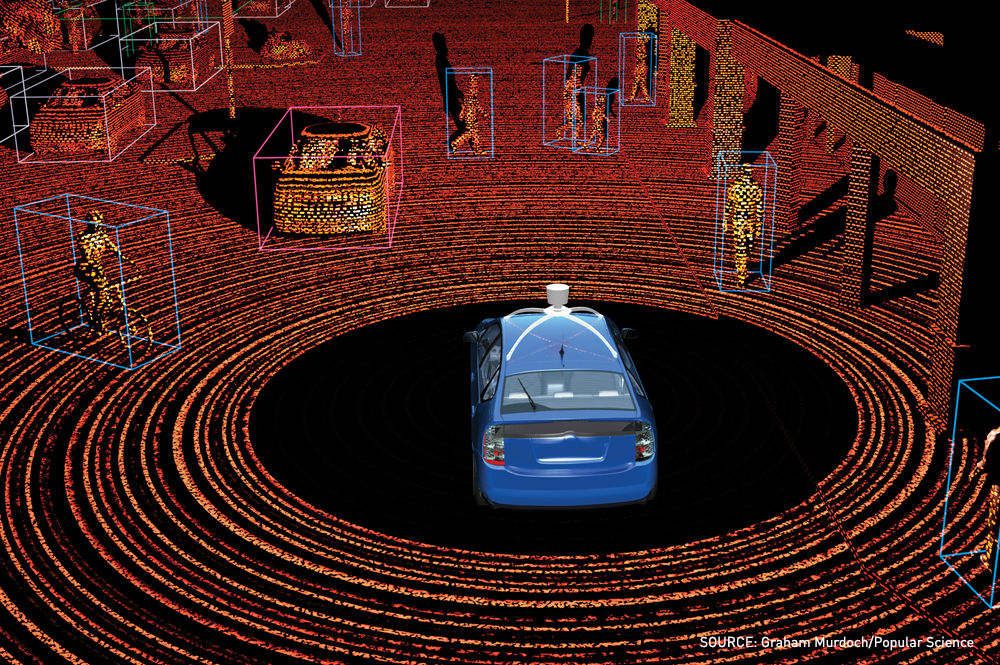
\includegraphics[width=6cm]{lidar_selfdrivingcar.png}
  \caption{Image fait avec LIDAR}
  \end{figure}
\end{frame}




\section{Microcontrôleur, nano-ordinateur, ordinateur : le cerveau du robot}
\subsection{Microcontrôleurs}
\begin{frame}
\frametitle{Définition}
\begin{block}{Définition}
Un microcontrôleur est un circuit intégré qui rassemble les éléments essentiels d'un ordinateur.
 Les microcontrôleurs se caractérisent par un plus haut degré d'intégration, une plus faible consommation électrique, une vitesse de fonctionnement plus faible  et un coût réduit par rapport aux microprocesseurs  utilisés dans les ordinateurs personnels. 
\end{block}
\end{frame}

\begin{frame}
\frametitle{Composition d'un microcontrôleur}
  Les composants d'un microcontrôleur sont :
  \begin{itemize}
      \item Un processeur ou un microprocesseur ARM\footnote{Dotés d'une architecture relativement plus simple que d'autres familles de processeurs, et bénéficiant d'une faible consommation électrique }.
      \item De la mémoire vive (RAM) 
      \item De la mémoire morte (ROM) 	
      \item Des périphériques, capables d'effectuer des tâches spécifiques\footnote{Watchdog, CAN,CNA}.
  \end{itemize}
\end{frame}


\begin{frame}
\frametitle{Exemple d'un microcontôleur}
\begin{figure}[!h]
\centering
\includegraphics[width=6cm]{expose.jpg}
\caption{Arduino, une carte construite autour d'un  microcontrôleur}
\end{figure}
\end{frame}


\begin{frame}
\frametitle{Programmation d'un microcontrôleur}
\begin{itemize}
\item À l'origine, les microcontrôleurs se programmaient en assembleur (problèmes de maintenance).
\item Désormais, on utilise de plus en plus des langages de haut niveau, notamment le langage C.
\item Avec l’augmentation de la puissance et de la quantité de mémoire de stockage , les programmes  peuvent désormais être écrits en C++. 
\item Il existe même des frameworks et plateformes en C++ destinés à l’embarqué, comme Qtopia, mais l'utilisation de ceux-ci restera limitée aux microcontrôleurs les plus puissants. 
\end{itemize}
\end{frame}
\begin{frame}
\begin{figure}[!h]
\centering
\includegraphics[width=6cm]{arduino.png}
\caption{Arduino IDE,l'IDE pour Arduino}
\end{figure}
\end{frame}
\begin{frame}
\begin{alertblock}{Ce qu'il faut retenir}
Adapté a un robot monotâche\\
Adapté a tout public (niveau de difficulté varié)\\
Programmable via différents langages informatique\\
Peu onéreux\footnote{Echelle de prix variant de 20 à 100 euros en moyenne}\\
Peu puissant\footnote{Mis a part quelques microcontrôleurs}\\
IDE fourni par le constructeur
\end{alertblock}
\begin{exampleblock}{Domaines d'applications}
Robotique domestque : tondeuse,aspirateur...\\
Très utilisé dans la robotique amateur \\
Robotique mobile\\
Petits robots humanoïdes
\end{exampleblock}
\end{frame}

\subsection{Nano-ordinateurs, ordinateurs mono-carte}

\begin{frame}
\frametitle{Définition}
 \begin{block}{Définition}
 Un ordinateur à carte unique ou ordinateur mono-carte est un ordinateur complet construit sur un circuit imprimé,
 avec un ou plusieurs microprocesseur(s), de la mémoire, des lignes d'entrée/sortie et d'autres éléments pour en faire un ordinateur fonctionnel. 
 \end{block}
\end{frame}


\begin{frame}
\frametitle{Exemple de nano-ordinateur}
\begin{figure}[!h]
\centering
\includegraphics[width=6cm]{BANANA_PI_01.jpg}
\caption{Un nano ordinateur, le banana PI}
\end{figure}
\end{frame}
\begin{frame}
\frametitle{Nano ordinateur ou microcontrôleur?}
\begin{itemize}
\item Si un nano-ordinateur a l’apparence d’un microcontrôleur, il :
\begin{itemize}
    \item Permet de faire fonctionner un système d’exploitation de haut niveau, comme par exemple Android ou Linux .
    \item Intègre ou il permet de connecter à minima des périphériques d’affichage (écran, télévision) et de saisie (clavier physique ou virtuel, souris ou écran tactile).
    \item Comporte un moyen de stockage dédié (disque dur, carte SD, clé usb) et possède un port ethernet.
    \item Fonctionne de manière autonome, sans nécessité de le raccorder à un autre ordinateur.
   \item Jusqu'a 40 fois plus rapide qu'un microcontroleur
\end{itemize}
\end{itemize}
\end{frame} 


\begin{frame}
\frametitle{Programmation d'un nano-ordinateur}
\begin{itemize}
    \item Au niveau de la programmation le nano-ordinateur pourra etre programmé dans n'importe quel langage de haut niveau et l'environnement de développement pourra être choisi car il comporte son propre système d'exploitation a contrario du microcontrôleur.
\end{itemize}
\end{frame}	

\begin{frame}
\begin{alertblock}{Ce qu'il faut retenir}
Adapté à un robot multitâches\\
Conçu pour un usage polyvalent\\
Adapté à tout public (niveau de difficulté varié)\\
Programmable via différents langages informatiques\\
Peu onéreux\\
Plus puissant qu'un microcontrôleur
\end{alertblock}
\begin{exampleblock}{Domaines d'applications}
Robotique mobile\\
Robotique domestique\\
Robotique DIY\\
Rontoique industrielle
\end{exampleblock}
\end{frame}


\subsection{Ordinateurs}
\begin{frame}
\begin{itemize}
\frametitle{Définition}
\item Depuis peu le constructeur NVIDIA a sorti le premier ordinateur spécialement concu pour la robotique le JETSON : équipé de neuf milliards de transistors et delivrant une puissance de calcul de 32 TOPS pour les calculs deep learning.
\item Il accélère les systèmes robotiques avec six unités de traitement à hautes performances : une puce graphique avec une architecture NVIDIA Volta à 512 cœurs, un processeur Carmel ARM64 à 8 cœurs, un double accélérateur NVDLA pour le Deep Learning, et des processeurs dédiés d’image, de vision et de vidéo.
\item Les ordinateurs dans la robotique ne datent pas d'aujourd'hui, plus puissants ils sont bien plus adaptés pour les applications industrielles.
\end{itemize}
\end{frame}
\begin{frame}
\frametitle{Exemple d'un ordinateur : Le Jetson}
\begin{figure}[!h]
\centering
\includegraphics[width=6cm]{jetson.jpg}
\caption{JETSON le premier ordinateur IA pour la robotique}
\end{figure}
\end{frame}
\begin{frame}
\frametitle{Programmation d'un Jetson}
\begin{itemize}
\item Ces nouveaux ordinateurs sont fournis avec un kit SDK  et integrent meme un IDE qui est une modification d'eclipse par NVIDIA et qui a été specialement concu pour ce type d'ordinateurs.
\item Le langage utilisé pour ces ordinateurs est le C, le C++  ou le Fortran\footnote{Fortran (FORmula TRANslator) est un langage de programmation utilisé principalement pour le calcul scientifique} car ce sont des langages puissants fait pour fonctionner avec CUDA\footnote{Architecture de traitement parallèle développée par NVIDIA permettant de décupler les performances de calcul du système en exploitant la puissance des processeurs graphiques }.
\end{itemize}
\end{frame}
\begin{frame}
\begin{figure}[!h]
\centering
\includegraphics[width=10cm]{NSIGH.png}
\caption{NSIGHT, l'IDE conçu pour le JETSON}
\end{figure}
\end{frame}
\begin{frame}
\frametitle{Conclusion}
\begin{alertblock}{Ce qu'il faut retenir}
Certains sont spécialement conçu pour la robotique\\
Adapté aux entreprises, laboratoires\\
Fait pour des professionels\\
Très puissant\footnote{Jeston est équivalent a une workstation GPU}\\
Onéreux en général
\end{alertblock}
\begin{exampleblock}{Domaines d'applications}
Médecine\\
Transport (robots livreurs)\\
Surveillance\\
Espace (Curiosity embarque deux ordinateurs !)\\
Robot humanoïdes
\end{exampleblock}
\end{frame}
\subsection{Conclusion}
\begin{frame}
\frametitle{Conclusion}
\begin{itemize}
\item En fonction du domaine d'application le choix du centre névralgique sera vite effectué
\item Les ordinateurs se repandent de plus en plus aujourd'hui dans la robotique et sont fait pour de vastes domaines d'applications dans le monde industriel jusqu'au voitures autonomes.
\item Il ne faut pas oublier que ces derniers sont faits pour des gens très experimentés contrairement a un microcontroleur ou un nano ordinateur.
\end{itemize}
\end{frame}
\begin{frame}
\begin{itemize}
\item Au final le choix du cerveau sera effectué en fonction du niveau de la ou les personne(s) qui concoivent le robot et aussi les besoins du robots. Pour des besoins industriels on peut dire que c'est surtout les ordinateurs qui sont employés car ils sont plus puissants.
\item Le langage C est le langage de prédilection pour la robotique avancée car c'est un langage très puissant.\footnote{Curiosity a été codé en C}.
\item Aujourd'hui les robots demandent de plus en plus de puissance notamment avec l'avancée de l'IA.
\end{itemize}
\end{frame}


\end{document} 
